\documentclass[a4paper,oneside]{book}

\usepackage{graphicx} % Allows insert of graphics
\usepackage{longtable} % Allows for multipage spanning tables
\usepackage{pdfpages} % Simplifies insertion of multipage PDF's
\usepackage{natbib} % Puts in bibliography style
\usepackage[pdfborder=0 0 0]{hyperref} % Adds PDF links
\usepackage{mathptm} % Changes font
\usepackage{fancyhdr} % Allows the use of the fancy Header package
\usepackage{url} % Makes URL's appear nicer and follow formatting rules
\usepackage[a4paper,vmargin={25.4mm,25.4mm},hmargin={25.4mm,25.4mm}]{geometry} % Allows the chaging of page borders

\setlength{\parindent}{0.0in} % Sets paragraph indentation to 0
\pagestyle{fancy}
\bibpunct{(}{)}{,}{a}{,}{,} % Defining the citation style
\newcommand{\degree}{\ensuremath{^\circ}} % Sets new command - Inserts degree symbol
\newcommand{\HRule}{\rule{\linewidth}{0.5mm}} % Set new command - Add blank line


\begin{document}
\chapter{Analysis}
\section{Fire Process}
Before starting analysis of the data, it is beneficial to discuss the fire process in more detail. A fire can occur within a building and is either started accidentally, be it through human error or a failure of some sort or the fire can be started deliberately (arson). Regardless of how it starts, a fire poses a threat to both the occupants and the property itself and measures are taken during the design and building process to minimise the risks to life safety.  This is the primary purpose of the design codes, which provide a set of guidelines that architects and designers are required to meet in the construction of the building. These systems are assumed to activate or provide protection during a fire incident, though the UK also maintains a fire and rescue service to provide assistance and fire-fighting capabilities for cases where these designed systems do not extinguish or contain the fire.
\\
\\
Most fires will follow the same process from start to finish. Figure \ref{fig:Fire_Process} shows this flow chart of how a fire progresses. 

\begin{figure}[htp]
\centering
	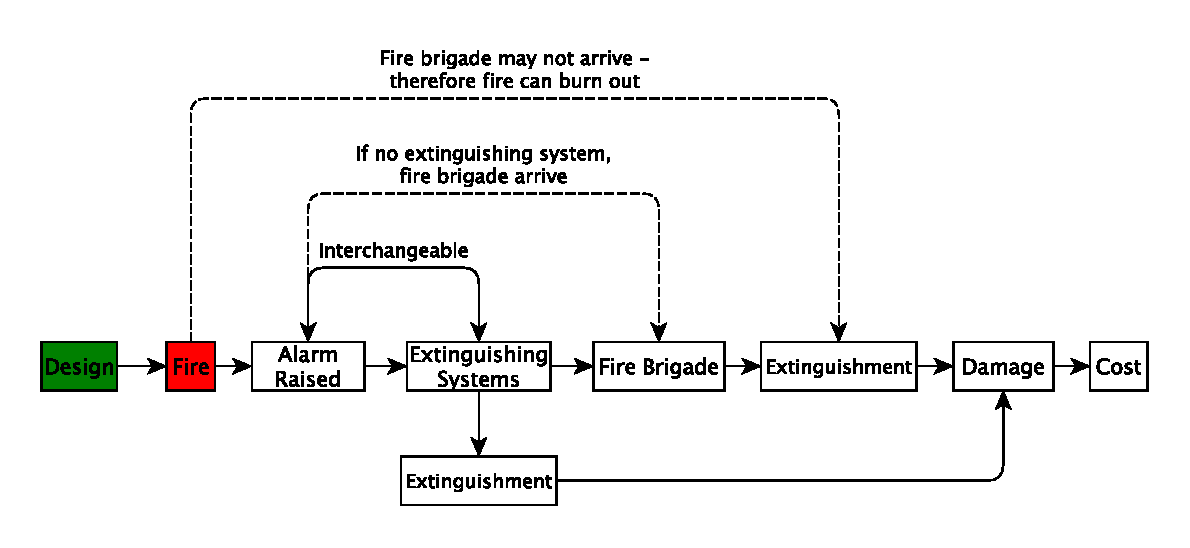
\includegraphics[width=14cm]{11-06-07_Fire_Process}
	\caption{Fire Process}
	\label{fig:Fire_Process}
\end{figure}

A building is initially designed with protection measures installed according to meeting the building regulations. These protection measures are specified in the design stage and this is the first step of the fire process. All buildings at one point were designed and a fire safety systems installed.
\\
The next stage is the fire itself. In this instance, we are assuming that the building in questions does have a fire - some buildings may last for the building lifetime without a fire. However, to demonstrate this fire process, a fire occurs.
\\
\\


\section{FDR 1 Data}
The FDR 1 data as described earlier in this thesis, is collected from fire incidents by fire fighters that attended the scene. This data was collected on paper forms after the incident occurs and was then later computerised. However, not all records were computerised - a sample was taken for each year (with the exception of 2005 in which all records were computerised).

\subsection{Alarms}

\section{FPA Data}
The data from the Fire Protection Association (FPA) is data collected from loss adjusters working for insurance companies. The electronic reporting system for this data has been in place since 2009 and the data in this dataset is all the data collected upto 24\textsuperscript{th} November 2010. Data in this database is only collected and stored if the fire estimated to have caused at least \pounds 100,000 worth of damage or if a fatality occurred in the fire. During the collection period, 963 incidents were collected and stored. However, of these, not all were caused by fires - some were caused by explosions. These were removed from the dataset as this work only details work where the fire was the cause of the incident. The dataset also contained data on residential buildings. As this is not part of the scope of this research, these were also removed. This left 650 records which can be broken down into the occupancy types detailed in Table \ref{tab:Incident_Frequency}.
\\
\\
The dataset was in the form of a comma separated value (CSV) file. Data was removed using a mixture of filtering in the Windows program CSVed (\url{http://csved.sjfrancke.nl/}) and by using the Linux programs \textit{awk} and \textit{sed} (which are also available for Windows). SPSS (\url{http://www.spss.com/} was also used for later analysis. Initially, it wasn't used due to producing errors from the dataset - however this was found to be caused by a corrupted data file that had been imported into the program and thus after this had been identified, the data was corrected according to the original data file provided by the FPA and the program was used in further data analysis.
\begin{table}[htbp]
	\centering
	\begin{tabular}{|l|c|c|c|}
	\hline
	\textbf{Occupancy}	&\textbf{Frequency}	&\textbf{Percent}	&\textbf{Cumulative Percent}	\\
	\hline
	Industrial Processing	&140	&21.5	&21.5	\\
	Non Residential -Misc	&107	&16.5	&38.0	\\
	Food and Drink	&89	&13.7	&51.7	\\
	Retail	&81	&12.5	&64.2	\\
	Warehouses	&64	&9.8	&74.0	\\
	Unassigned	&29	&4.5	&78.5	\\
	Permanent Agricultural	&27	&4.2	&82.6	\\
	Education	&24	&3.7	&86.3	\\
	Entertainment and Culture	&24	&3.7	&90.0	\\
	Religious	&23	&3.5	&93.5	\\
	Sport	&19	&2.9	&96.5	\\
	Medical	&9	&1.4	&97.8	\\
	Transport	&5	&0.8	&98.6	\\
	Outdoor structures	&3	&0.5	&99.1	\\
	Car Parks	&2	&0.3	&99.4	\\
	Other outdoors (including land)	&2	&0.3	&99.7	\\
	Outdoor equipment and machinery	&1	&0.2	&99.8	\\
	Public Utilities	&1	&0.2	&100.0	\\
	\hline
	\textbf{Total}	&650	&100	&	\\
	\hline
	\end{tabular}
	\caption{Frequencies of Incidents per Occupancy Type}
	\label{tab:Incident_Frequency}
\end{table}

\subsection{Rateable Values}
Rateable values can provide a baseline figure to the cost of the fire - rateable values are the cost values at which a property might be expected to be let for one year \citep{ValuationOfficeAgency2008}. Therefore if damage occurs as a result of a fire, then the area damaged incurs a loss, either through the lack of rent or from the inability to use that area until it is repaired (for instances where the building occupiers also own the building). By using this value, a baseline estimate of the cost of damage can be calculated. It is expected that the costs of a fire will be greater than the rateable value as the fire will consume items within the property as fuel and these items are not taken into account in the rateable value.
\\
\\
The rateable values given by the Office of National Statistics (ONS) and the Valuation Office Agency (VOA) are split into the following categories:-
\begin{itemize}
\item Retail - Sells goods or services to the public i.e. post offices, restaurants, shops. Excludes pubs.
\item Office - This is further split down into the following:
\begin{enumerate}
\item Commercial Offices - Purpose built offices and offices above shops etc.
\item Other - Includes offices such as local government offices and police stations. Includes some surgeries and clinics.
\end{enumerate}
\item Factories - Includes small workshops and large manufacturing units
\item Warehouses - Small storage units upto large warehouses. Car show rooms are classed as warehouses.
\item Other Bulk - Premises that don't fall into one above - i.e. garden centres, halls and social clubs.
\item Non Bulk - Most prevalent are pubs, advertising rights, car parks and holiday homes.
\end{itemize}
Some properties are exempt from rateable values, such as churches (and other religious buildings), parks and agricultural buildings.
\\
\\


\clearpage
\addcontentsline{toc}{section}{Bibliography}
\bibliographystyle{custom}
\bibliography{../../Bibliography}

\end{document}
